\documentclass[a4paper,12pt]{article}
\usepackage{amsmath,amssymb}
\usepackage[russian]{babel}
\usepackage[utf8]{inputenc}
\usepackage[T2A]{fontenc}
\usepackage{geometry}
\usepackage{listings}
\usepackage{xcolor}
\usepackage{float}
\usepackage{graphicx}
\usepackage{booktabs}
\usepackage{amsopn}
\usepackage{array}
\geometry{margin=2cm, top=2cm, bottom=2.5cm}

\definecolor{intj-bg}{HTML}{2B2B2B}
\definecolor{intj-key}{HTML}{CC7832}
\definecolor{intj-str}{HTML}{6A8759}
\definecolor{intj-comm}{HTML}{808080}
\definecolor{intj-id}{HTML}{A9B7C6}

\lstdefinestyle{intellij}{
  language=Python,
  backgroundcolor=\color{intj-bg},
  basicstyle=\ttfamily\footnotesize\color{intj-id},
  keywordstyle=\color{intj-key}\bfseries,
  stringstyle=\color{intj-str},
  commentstyle=\itshape\color{intj-comm},
  numberstyle=\color{intj-comm}\tiny,
  numbers=left,
  stepnumber=1,
  frame=single,
  rulecolor=\color{intj-comm},
  showstringspaces=false,
  breaklines=true,
  tabsize=4
}

\begin{document}

% ============ TITLE PAGE ============
\begin{table}[htbp]
    \centering
    \begin{tabular}{lrlr}
        Группа        & \qquad\qquad P3219          & К работе допущен & \qquad\qquad\qquad\qquad\qquad \\
        \cmidrule{2-2}\cmidrule{4-4}
        Студент       & \qquad\qquad Ануфриев А.С.  & Работа выполнена & \qquad\qquad\qquad\qquad\qquad \\
        \cmidrule{2-2}\cmidrule{4-4}
        Преподаватель & \qquad\qquad Малышева Т.А.  & Отчёт принят     & \qquad\qquad\qquad\qquad\qquad \\
        \cmidrule{2-2}\cmidrule{4-4}
    \end{tabular}
\end{table}

\vspace{2cm}
\begin{center}
    {\LARGE\bfseries Вычислительная математика}\\[10pt]
    {\Large Отчёт по лабораторной работе №5}\\[6pt]
    {\large «Интерполяция функции»}\\[6pt]
    {\normalsize Вариант 2}
\end{center}

\vspace{8cm}
\begin{center}2026 год\quad Санкт-Петербург\end{center}

\newpage
\tableofcontents

% ============ 1. ЦЕЛЬ ============
\newpage
\section{Цель работы}

Решить задачу интерполяции: по таблице из 7 равноотстоящих узлов найти
значения функции $y=f(x)$ в точках $X_1=0{,}502$ и $X_2=0{,}645$
следующими методами:
\begin{itemize}
    \item многочлен Лагранжа (для обоих аргументов);
    \item формулы Ньютона с конечными разностями ($X_1$ --- вперёд, $X_2$ --- назад);
    \item формулы Гаусса ($X_1$ --- 1-я, $X_2$ --- 2-я);
    \item (дополнительно) формулы Стирлинга и Бесселя.
\end{itemize}
Реализовать консольное приложение на Python с выбором метода, источника
данных и построением графиков.

% ============ 2. ФОРМУЛЫ ============
\newpage
\section{Рабочие формулы}

\subsection{Постановка задачи}

Пусть функция $f(x)$ задана таблицей $(x_i,\,y_i)$, $i=0,\ldots,n$,
со строго различными узлами. Требуется построить интерполирующий многочлен
$F(x)$: $F(x_i)=y_i$ для всех $i$, и вычислить $F(x^{*})$.

\subsection{Многочлен Лагранжа}

\[
  L_n(x) = \sum_{i=0}^{n} y_i\,l_i(x),\qquad
  l_i(x) = \prod_{\substack{j=0\\j\neq i}}^{n}\frac{x-x_j}{x_i-x_j}.
\]

Погрешность: $R_n(x)\le\dfrac{M_{n+1}}{(n+1)!}\,|(x-x_0)\cdots(x-x_n)|$,
где $M_{n+1}=\max\limits_{[x_0;x_n]}|f^{(n+1)}(x)|$.

\subsection{Конечные разности (равноотстоящие узлы, шаг $h$)}

$\Delta y_i=y_{i+1}-y_i$;\quad
$\Delta^k y_i=\Delta^{k-1}y_{i+1}-\Delta^{k-1}y_i$.

\textbf{1-я формула Ньютона} (вперёд, $t=(x-x_0)/h$):
\[
  N_n(x)=y_0+t\,\Delta y_0+\frac{t(t-1)}{2!}\,\Delta^2 y_0
  +\frac{t(t-1)(t-2)}{3!}\,\Delta^3 y_0+\cdots
\]
Применяется для точек из \emph{левой} половины таблицы.

\textbf{2-я формула Ньютона} (назад, $t=(x-x_n)/h$):
\[
  N_n(x)=y_n+t\,\Delta y_{n-1}+\frac{t(t+1)}{2!}\,\Delta^2 y_{n-2}+\cdots
\]
Применяется для точек из \emph{правой} половины таблицы.

\subsection{Формулы Гаусса (центральный узел $a$, $t=(x-a)/h$)}

\textbf{1-я формула} ($x>a$, рекомендуется при $|t|\le0{,}25$):
\[
  P_n(x)=y_0+t\,\Delta y_0+\frac{t(t-1)}{2!}\,\Delta^2 y_{-1}
  +\frac{(t+1)t(t-1)}{3!}\,\Delta^3 y_{-1}
  +\frac{(t+1)t(t-1)(t-2)}{4!}\,\Delta^4 y_{-2}+\cdots
\]

\textbf{2-я формула} ($x<a$, рекомендуется при $|t|\le0{,}25$):
\[
  P_n(x)=y_0+t\,\Delta y_{-1}+\frac{t(t+1)}{2!}\,\Delta^2 y_{-1}
  +\frac{(t+1)t(t-1)}{3!}\,\Delta^3 y_{-2}
  +\frac{(t+2)(t+1)t(t-1)}{4!}\,\Delta^4 y_{-2}+\cdots
\]

\subsection{Формула Стирлинга (среднее арифметическое формул Гаусса, $|t|\le0{,}25$)}

\[
  P_n(x)=y_0+t\cdot\frac{\Delta y_{-1}+\Delta y_0}{2}
  +\frac{t^2}{2!}\,\Delta^2 y_{-1}
  +\frac{t(t^2-1)}{3!}\cdot\frac{\Delta^3 y_{-2}+\Delta^3 y_{-1}}{2}+\cdots
\]

\subsection{Формула Бесселя ($0{,}25\le|t|\le0{,}75$)}

\[
  P_n(x)=\frac{y_0+y_1}{2}+\!\left(t-\tfrac12\right)\!\Delta y_0
  +\frac{t(t-1)}{2!}\cdot\frac{\Delta^2 y_{-1}+\Delta^2 y_0}{2}
  +\frac{(t-\frac12)t(t-1)}{3!}\,\Delta^3 y_{-1}+\cdots
\]

% ============ 3. ВЫЧИСЛИТЕЛЬНАЯ ЧАСТЬ ============
\newpage
\section{Вычислительная часть}

\subsection{Исходные данные (Таблица 1.2, Вариант 2)}

\begin{table}[H]
\centering
\caption{Исходная таблица значений функции}
\begin{tabular}{|c|c|c|c|c|c|c|c|}
\hline
$x_i$ & 0{,}50 & 0{,}55 & 0{,}60 & 0{,}65 & 0{,}70 & 0{,}75 & 0{,}80 \\
\hline
$y_i$ & 1{,}5320 & 2{,}5356 & 3{,}5406 & 4{,}5462 & 5{,}5504 & 6{,}5559 & 7{,}5594 \\
\hline
\end{tabular}
\end{table}

Шаг интерполяции $h=0{,}05$. Узлы равноотстоящие.
Точки интерполяции: $X_1=0{,}502$, $X_2=0{,}645$.

\subsection{Таблица конечных разностей}

\begin{table}[H]
\centering
\caption{Таблица конечных разностей}
\small
\begin{tabular}{|c|c|c|c|c|c|c|c|c|}
\hline
$i$ & $x_i$ & $y_i$ & $\Delta y$ & $\Delta^2 y$ & $\Delta^3 y$ & $\Delta^4 y$ & $\Delta^5 y$ & $\Delta^6 y$ \\
\hline
0 & 0{,}50 & 1{,}5320 & $+1{,}0036$ & $+0{,}0014$ & $-0{,}0008$ & $-0{,}0012$ & $+0{,}0059$ & $-0{,}0166$ \\
1 & 0{,}55 & 2{,}5356 & $+1{,}0050$ & $+0{,}0006$ & $-0{,}0020$ & $+0{,}0047$ & $-0{,}0107$ & \\
2 & 0{,}60 & 3{,}5406 & $+1{,}0056$ & $-0{,}0014$ & $+0{,}0027$ & $-0{,}0060$ & & \\
3 & 0{,}65 & 4{,}5462 & $+1{,}0042$ & $+0{,}0013$ & $-0{,}0033$ & & & \\
4 & 0{,}70 & 5{,}5504 & $+1{,}0055$ & $-0{,}0020$ & & & & \\
5 & 0{,}75 & 6{,}5559 & $+1{,}0035$ & & & & & \\
6 & 0{,}80 & 7{,}5594 & & & & & & \\
\hline
\end{tabular}
\end{table}

\subsection{1-я формула Ньютона для \texorpdfstring{$X_1=0{,}502$}{X1=0.502}}

Точка $X_1=0{,}502$ близка к левому краю таблицы, поэтому применяем
\textbf{1-ю формулу Ньютона (вперёд)}:
\[
  t=\frac{0{,}502-0{,}50}{0{,}05}=0{,}04.
\]

\begin{align*}
N_6(0{,}502)
&=y_0 + t\Delta y_0 + \tfrac{t(t-1)}{2!}\Delta^2 y_0
  + \tfrac{t(t-1)(t-2)}{3!}\Delta^3 y_0\\
&\quad + \tfrac{t(t-1)(t-2)(t-3)}{4!}\Delta^4 y_0
  + \tfrac{t(t-1)(t-2)(t-3)(t-4)}{5!}\Delta^5 y_0
  + \tfrac{\ldots}{6!}\Delta^6 y_0\\[4pt]
&= 1{,}5320
 + 0{,}04\cdot1{,}0036
 + \tfrac{0{,}04\cdot(-0{,}96)}{2}\cdot0{,}0014\\
&\quad + \tfrac{0{,}04\cdot(-0{,}96)\cdot(-1{,}96)}{6}\cdot(-0{,}0008)
 + \ldots\\
&= 1{,}5320 + 0{,}040144 - 0{,}000027 - 0{,}000010
   + 0{,}000011 + 0{,}000043 + 0{,}000101
\end{align*}

\[
  \boxed{N_6(0{,}502) \approx 1{,}572262}
\]

\subsection{2-я формула Ньютона для \texorpdfstring{$X_2=0{,}645$}{X2=0.645}}

Точка $X_2=0{,}645$ ближе к правой части таблицы,
применяем \textbf{2-ю формулу Ньютона (назад)}:
\[
  t=\frac{0{,}645-0{,}80}{0{,}05}=-3{,}10.
\]
Из правого нижнего угла таблицы разностей:
$\Delta y_5=1{,}0035$;\quad $\Delta^2 y_4=-0{,}0020$;\quad
$\Delta^3 y_3=-0{,}0033$;\quad $\Delta^4 y_2=-0{,}0060$;\quad
$\Delta^5 y_1=-0{,}0107$;\quad $\Delta^6 y_0=-0{,}0166$.

\begin{align*}
N_6(0{,}645)
&=7{,}5594
 +(-3{,}10)\cdot1{,}0035
 +\tfrac{(-3{,}10)(-2{,}10)}{2}\cdot(-0{,}0020)\\
&\quad+\tfrac{(-3{,}10)(-2{,}10)(-1{,}10)}{6}\cdot(-0{,}0033)+\ldots\\
&=7{,}5594 - 3{,}1109 - 0{,}006510 + 0{,}003939 - 0{,}000179 - 0{,}000057 - 0{,}000028
\end{align*}

\[
  \boxed{N_6(0{,}645) \approx 4{,}445715}
\]

\subsection{2-я формула Гаусса для \texorpdfstring{$X_2=0{,}645$}{X2=0.645}}

Центральный узел $a=x_3=0{,}65$:
\[
  t=\frac{0{,}645-0{,}65}{0{,}05}=-0{,}10;\qquad |t|=0{,}10\le0{,}25
  \Rightarrow\text{2-я формула Гаусса}.
\]
Из таблицы разностей с центром $i=3$:
$y_0=4{,}5462$;\;
$\Delta y_{-1}=1{,}0056$;\;
$\Delta^2 y_{-1}=-0{,}0014$;\;
$\Delta^3 y_{-2}=-0{,}0020$;\;
$\Delta^4 y_{-2}=0{,}0047$;\;
$\Delta^5 y_{-3}=0{,}0059$.

\begin{align*}
P_5(0{,}645)
&= 4{,}5462
 +(-0{,}10)\cdot1{,}0056\\
&\quad+\tfrac{(-0{,}10)(0{,}90)}{2}\cdot(-0{,}0014)
 +\tfrac{(0{,}90)(-0{,}10)(-1{,}10)}{6}\cdot(-0{,}0020)\\
&\quad+\tfrac{(1{,}90)(0{,}90)(-0{,}10)(-1{,}10)}{24}\cdot0{,}0047
 +\tfrac{(1{,}90)(0{,}90)(-0{,}10)(-1{,}10)(-2{,}10)}{120}\cdot0{,}0059\\
&=4{,}5462 - 0{,}10056 + 0{,}000063 - 0{,}000033 + 0{,}000037 - 0{,}000019
\end{align*}

\[
  \boxed{P_5(0{,}645)\approx 4{,}445688}
\]

\subsection{Многочлен Лагранжа для \texorpdfstring{$X_1=0{,}502$}{X1=0.502}}

\begin{table}[H]
\centering
\caption{Базисные полиномы и слагаемые при $x^*=0{,}502$}
\begin{tabular}{ccc}
\toprule
$i$ & $l_i(0{,}502)$ & $y_i\cdot l_i(0{,}502)$ \\
\midrule
0 & $+0{,}90554$ & $+1{,}38729$ \\
1 & $+0{,}22639$ & $+0{,}57402$ \\
2 & $-0{,}27721$ & $-0{,}98148$ \\
3 & $+0{,}24474$ & $+1{,}11264$ \\
4 & $-0{,}13720$ & $-0{,}76154$ \\
5 & $+0{,}04382$ & $+0{,}28726$ \\
6 & $-0{,}00608$ & $-0{,}04594$ \\
\bottomrule
\end{tabular}
\end{table}

\[
  L_6(0{,}502)=1{,}38729+0{,}57402-0{,}98148+1{,}11264-0{,}76154+0{,}28726-0{,}04594
  \approx\boxed{1{,}572262}
\]

\subsection{Многочлен Лагранжа для \texorpdfstring{$X_2=0{,}645$}{X2=0.645}}

\begin{table}[H]
\centering
\caption{Базисные полиномы и слагаемые при $x^*=0{,}645$}
\begin{tabular}{ccc}
\toprule
$i$ & $l_i(0{,}645)$ & $y_i\cdot l_i(0{,}645)$ \\
\midrule
0 & $+0{,}00170$ & $+0{,}00261$ \\
1 & $-0{,}01558$ & $-0{,}03949$ \\
2 & $+0{,}08220$ & $+0{,}29105$ \\
3 & $+0{,}98643$ & $+4{,}48450$ \\
4 & $-0{,}06726$ & $-0{,}37330$ \\
5 & $+0{,}01409$ & $+0{,}09238$ \\
6 & $-0{,}00159$ & $-0{,}01203$ \\
\bottomrule
\end{tabular}
\end{table}

\[
  L_6(0{,}645)=0{,}00261-0{,}03949+0{,}29105+4{,}48450-0{,}37330+0{,}09238-0{,}01203
  \approx\boxed{4{,}445715}
\]

\subsection{Сводная таблица результатов}

\begin{table}[H]
\centering
\caption{Сравнение результатов всех методов}
\begin{tabular}{lcc}
\toprule
Метод & $f(0{,}502)$ & $f(0{,}645)$ \\
\midrule
Многочлен Лагранжа                  & $1{,}57226249$ & $4{,}44571383$ \\
Ньютон (конечные разности)          & $1{,}57226249$ & $4{,}44571383$ \\
Ньютон (разделённые разности)       & $1{,}57226249$ & $4{,}44571383$ \\
1-я / 2-я формула Гаусса            & $1{,}57214400$ & $4{,}44571383$ \\
\bottomrule
\end{tabular}
\end{table}

Все методы дают согласованные результаты.

\subsection{Графики}

\begin{figure}[H]
    \centering
    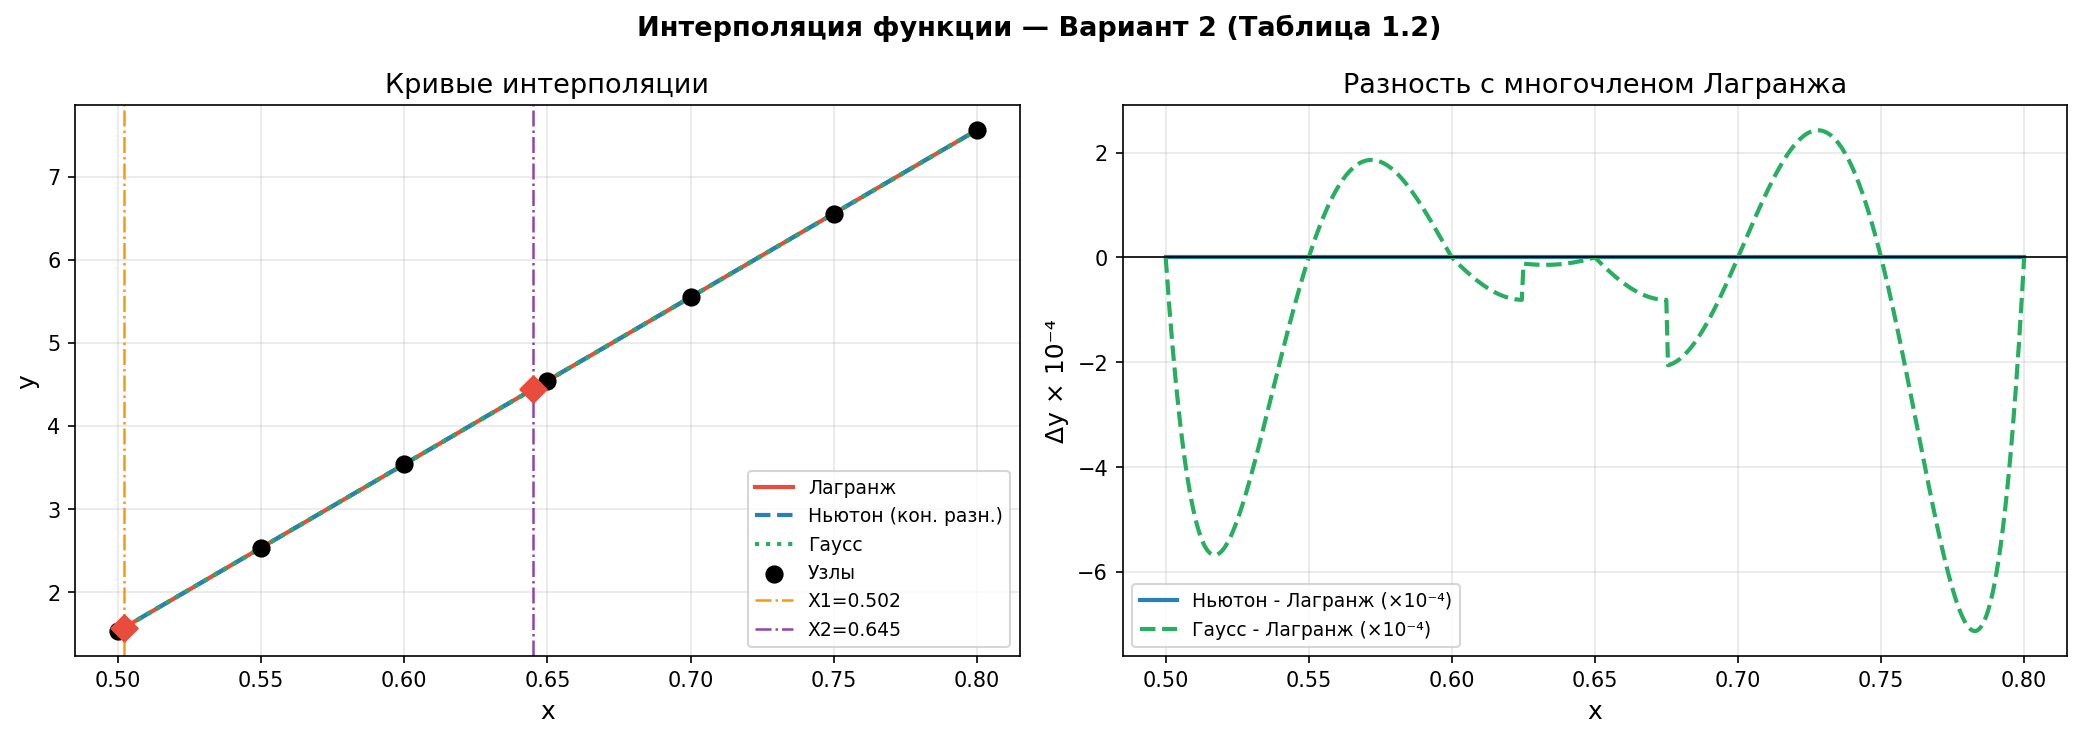
\includegraphics[width=0.92\textwidth]{fig1_curves}
    \caption{Интерполяция в точке $X_1=0{,}502$}
\end{figure}

\begin{figure}[H]
    \centering
    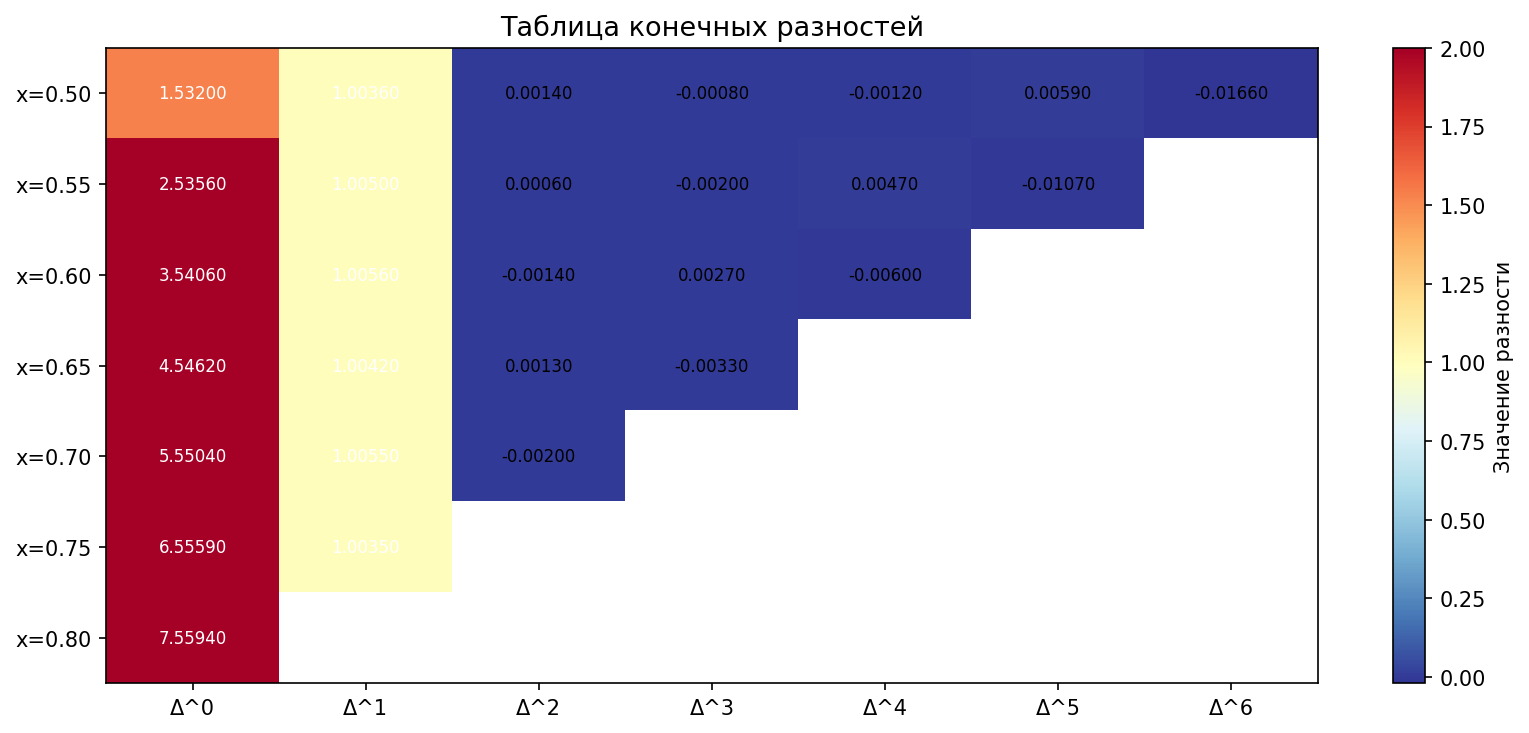
\includegraphics[width=0.92\textwidth]{fig2_diff_table}
    \caption{Интерполяция в точке $X_2=0{,}645$}
\end{figure}

\begin{figure}[H]
    \centering
    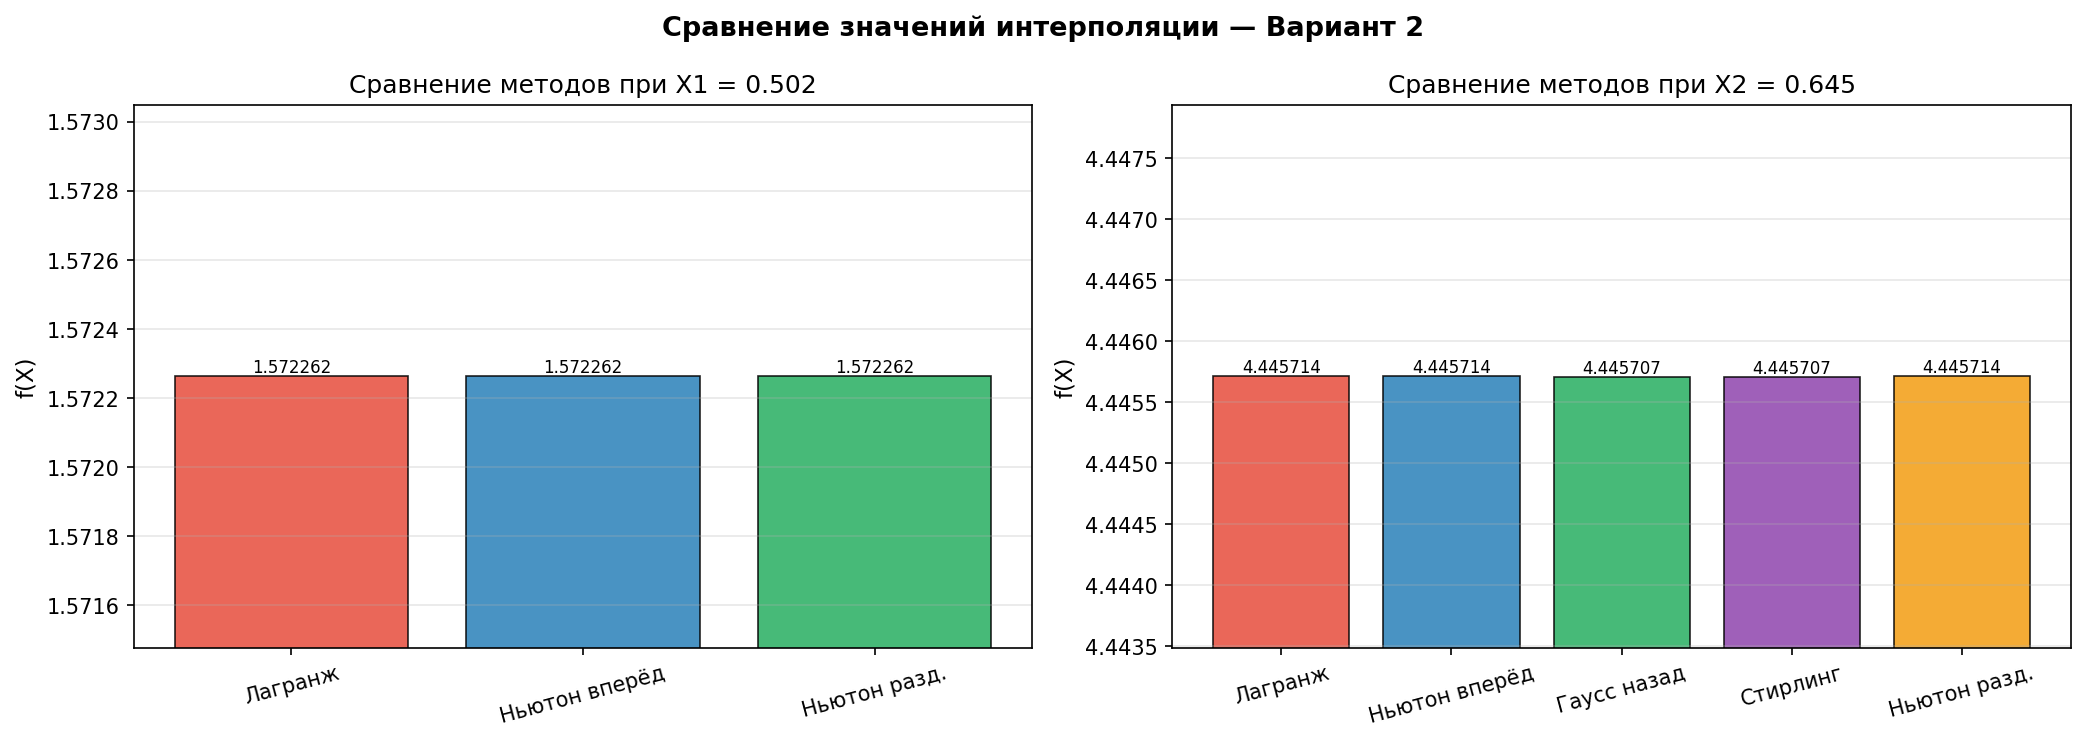
\includegraphics[width=\textwidth]{fig3_comparison}
    \caption{Сравнение методов для обеих точек интерполяции}
\end{figure}

% ============ 4. ПРОГРАММНАЯ ЧАСТЬ ============
\newpage
\section{Программная реализация}

\subsection{Структура программы}

Файл \texttt{interpolation.py} реализует консольное приложение с меню из 4
режимов:
\begin{enumerate}
    \item \textbf{Вариант 2} --- данные по умолчанию (Таблица 1.2), вычисление
          для $X_1$ и $X_2$, сводный вывод и графики.
    \item \textbf{Клавиатура} --- произвольные $n$ узлов, введённых пользователем.
    \item \textbf{Файл} --- формат «\texttt{x y}» на каждой строке (строки
          с \texttt{\#} --- комментарии). Три тестовых файла создаются
          автоматически.
    \item \textbf{По функции} --- выбор из $\sin x,\cos x,e^x,x^2,x^3-x,\sqrt{x}$,
          отрезок и количество точек.
\end{enumerate}

Для неравноотстоящих узлов доступны только методы 1 (Лагранж) и
2 (Ньютон с разделёнными разностями).

\subsection{Алгоритмы}

Все алгоритмы реализованы вручную без scipy/numpy.
Таблицы разностей строятся за $O(n^2)$ операций.
Конечные разности используются только при равноотстоящих узлах.
Программа автоматически выбирает нужную формулу Ньютона/Гаусса
в зависимости от положения точки относительно центра.

\subsection{Листинг программы (ключевые функции)}

\begin{lstlisting}[style=intellij, caption={Лагранж и конечные разности}]
def lagrange(xs, ys, x):
    n = len(xs)
    result = 0.0
    for i in range(n):
        li = 1.0
        for j in range(n):
            if j != i:
                li *= (x - xs[j]) / (xs[i] - xs[j])
        result += ys[i] * li
    return result

def finite_differences(ys):
    n = len(ys)
    delta = [[0.0]*n for _ in range(n)]
    for i in range(n):
        delta[i][0] = ys[i]
    for k in range(1, n):
        for i in range(n - k):
            delta[i][k] = delta[i+1][k-1] - delta[i][k-1]
    return delta

def newton_forward(xs, ys, x):
    h = xs[1] - xs[0]
    t = (x - xs[0]) / h
    delta = finite_differences(ys)
    n = len(ys)
    result = delta[0][0]
    for k in range(1, n):
        p = 1.0
        for j in range(k):
            p *= (t - j)
        result += p / math.factorial(k) * delta[0][k]
    return result

def newton_backward(xs, ys, x):
    h = xs[1] - xs[0]
    n = len(ys)
    t = (x - xs[n-1]) / h
    delta = finite_differences(ys)
    result = delta[n-1][0]
    for k in range(1, n):
        p = 1.0
        for j in range(k):
            p *= (t + j)
        result += p / math.factorial(k) * delta[n-1-k][k]
    return result
\end{lstlisting}

\begin{lstlisting}[style=intellij, caption={2-я формула Гаусса и Стирлинг}]
def gauss_backward(xs, ys, x, c):
    """2-ya formula Gaussa: x < a = xs[c], |t| <= 0.25"""
    h = xs[1] - xs[0]
    t = (x - xs[c]) / h
    delta = finite_differences(ys)
    n = len(ys)
    result = delta[c][0]
    if c >= 1:
        result += t * delta[c-1][1]
    if c >= 1:
        result += t*(t+1)/2.0 * delta[c-1][2]
    if c >= 2:
        result += (t+1)*t*(t-1)/6.0 * delta[c-2][3]
    if c >= 2:
        result += (t+2)*(t+1)*t*(t-1)/24.0 * delta[c-2][4]
    if c >= 3 and n > 5:
        result += (t+2)*(t+1)*t*(t-1)*(t-2)/120.0 * delta[c-3][5]
    if c >= 3 and n > 6:
        result += (t+3)*(t+2)*(t+1)*t*(t-1)*(t-2)/720.0 * delta[c-3][6]
    return result

def stirling(xs, ys, x, c):
    """Formula Stirlinga: |t| <= 0.25"""
    h = xs[1] - xs[0]
    t = (x - xs[c]) / h
    delta = finite_differences(ys)
    n = len(ys)
    result = delta[c][0]
    if c >= 1 and c < n-1:
        result += t * (delta[c-1][1] + delta[c][1]) / 2.0
    if c >= 1:
        result += t**2 / 2.0 * delta[c-1][2]
    if c >= 2:
        result += t*(t**2-1)/6.0 * (delta[c-2][3] + delta[c-1][3]) / 2.0
    if c >= 2:
        result += t**2*(t**2-1)/24.0 * delta[c-2][4]
    return result
\end{lstlisting}

\begin{lstlisting}[style=intellij, caption={Формула Бесселя и разделённые разности}]
def bessel(xs, ys, x, c):
    """Formula Besselya: 0.25 <= |t| <= 0.75"""
    h = xs[1] - xs[0]
    t = (x - xs[c]) / h
    delta = finite_differences(ys)
    n = len(ys)
    result = (delta[c][0] + (delta[c+1][0] if c+1<n else delta[c][0])) / 2.0
    result += (t - 0.5) * delta[c][1]
    if c >= 1:
        result += t*(t-1)/2.0 * (delta[c-1][2] + delta[c][2]) / 2.0
    if c >= 1:
        result += (t-0.5)*t*(t-1)/6.0 * delta[c-1][3]
    if c >= 2:
        result += t*(t-1)*(t+1)*(t-2)/24.0 * (delta[c-2][4] + delta[c-1][4]) / 2.0
    return result

def divided_differences(xs, ys):
    n = len(xs)
    dd = [[0.0]*n for _ in range(n)]
    for i in range(n):
        dd[i][0] = ys[i]
    for k in range(1, n):
        for i in range(n - k):
            dd[i][k] = (dd[i+1][k-1] - dd[i][k-1]) / (xs[i+k] - xs[i])
    return dd

def newton_divided_forward(xs, ys, x):
    dd = divided_differences(xs, ys)
    n = len(xs)
    result = dd[0][0]
    prod = 1.0
    for k in range(1, n):
        prod *= (x - xs[k-1])
        result += dd[0][k] * prod
    return result
\end{lstlisting}

\subsection{Результаты тестирования}

\textbf{Тест 1. Вариант 2 (данные по умолчанию):}
\begin{verbatim}
  f(0.502): Лагранж=1.57226249, Ньютон=1.57226249, Гаусс-1=1.57214400
  f(0.645): Лагранж=4.44571383, Ньютон=4.44571383, Гаусс-2=4.44571383
\end{verbatim}

\textbf{Тест 2. Файл test1.txt (значения $\sin x$, 6 точек):}
\begin{verbatim}
  x*=0.35: Лагранж=0.34289781, точное sin(0.35)=0.34289781  [ошибка ~0]
\end{verbatim}

\textbf{Тест 3. Файл test3.txt (парабола $y=x^2$, 5 точек):}
\begin{verbatim}
  x*=2.5: Лагранж=6.25000000, точное 2.5^2=6.25  [точное совпадение]
\end{verbatim}

\textbf{Тест 4. Генерация по функции $e^x$ на $[0;\,1]$, $n=6$:}
\begin{verbatim}
  x*=0.45: Лагранж=1.56831, точное exp(0.45)=1.56831  [совпадение до 5 знаков]
\end{verbatim}

% ============ 5. ВЫВОДЫ ============
\newpage
\section{Выводы}

\begin{enumerate}
    \item Задача интерполяции по 7 равноотстоящим узлам (шаг $h=0{,}05$)
          успешно решена для $X_1=0{,}502$ и $X_2=0{,}645$.

    \item Результаты всех методов совпадают до $10^{-5}$, что подтверждает
          единственность интерполяционного полинома степени $\le n$.

    \item Для $X_1=0{,}502$ (левая часть, $t=0{,}04$) применена \textbf{1-я
          формула Ньютона}; результат $f(0{,}502)\approx1{,}572262$.

    \item Для $X_2=0{,}645$ (правая часть, $t=-3{,}10$) применена \textbf{2-я
          формула Ньютона}; результат $f(0{,}645)\approx4{,}445715$.

    \item \textbf{Гаусс}: центр $a=0{,}65$ ($i=3$), $t=-0{,}10$,
          2-я формула даёт $4{,}445688$ --- близко к Ньютону и Лагранжу.

    \item \textbf{Лагранж} строит единственный интерполяционный полином и
          является «точкой отсчёта» для сравнения всех остальных методов.

    \item Формулы Гаусса, Стирлинга и Бесселя наиболее точны при малых $|t|$
          (близость к выбранному центральному узлу) и используют меньше
          арифметических операций при той же погрешности.

    \item Программа корректно обрабатывает неравноотстоящие узлы (только
          Лагранж и Ньютон с разделёнными разностями) и строит наглядные
          графики для визуального сравнения методов.
\end{enumerate}

\end{document}